\section{Results – Strategy S2: Iterative Single-Field}
\label{sec:eval-s2}

The \textbf{S2: Iterative Single-Field} strategy fills the template sequentially, invoking the LLM once per slot. We evaluate three S2 variants: \textbf{S2.0} without few-shot examples on the original MUC-4 dataset, \textbf{S2.1} with few-shot examples on the original dataset, and \textbf{S2.2} with few-shot examples on a modified dataset that mimics speech-style transcripts.

\begin{figure}[H]
\centering
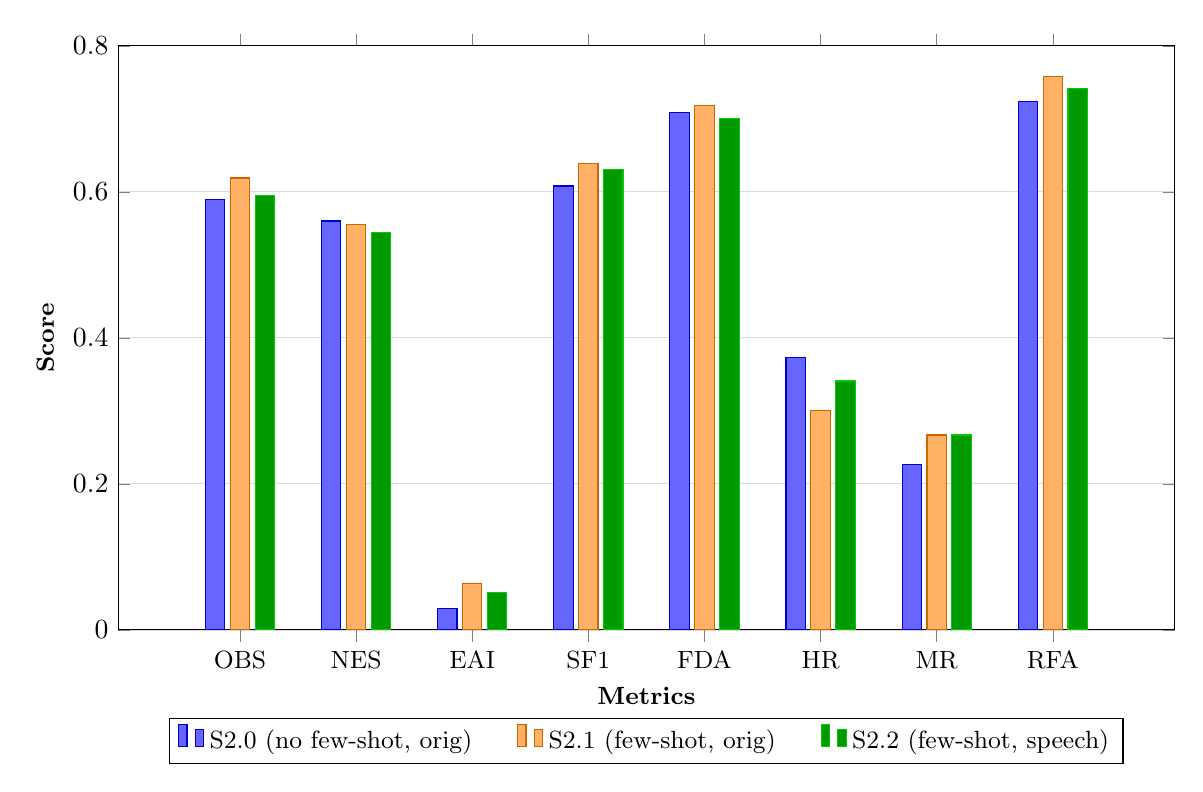
\begin{tikzpicture}
  \begin{axis}[
    width=15cm,
    height=9cm,
    ybar,
    bar width=7pt,
    ylabel={Score},
    ylabel style={font=\small\bfseries},
    xlabel={Metrics},
    xlabel style={font=\small\bfseries},
    symbolic x coords={OBS, NES, EAI, SF1, FDA, HR, MR, RFA},
    xtick=data,
    xticklabel style={font=\small},
    ymin=0,
    ymax=0.8,
    ytick={0, 0.2, 0.4, 0.6, 0.8},
    ymajorgrids=true,
    grid style={line width=0.3pt, draw=gray!30},
    legend style={
      at={(0.5,-0.15)},
      anchor=north,
      legend columns=3,
      font=\small,
      /tikz/every even column/.append style={column sep=0.5cm}
    },
    enlarge x limits=0.15,
  ]
  
  % S2.0 (no few-shot, orig) - Blue
  \addplot[fill=blue!60, draw=blue!80!black] coordinates {
    (OBS, 0.590)
    (NES, 0.560)
    (EAI, 0.029)
    (SF1, 0.608)
    (FDA, 0.709)
    (HR, 0.373)
    (MR, 0.226)
    (RFA, 0.724)
  };
  \addlegendentry{S2.0 (no few-shot, orig)}
  
  % S2.1 (few-shot, orig) - Orange
  \addplot[fill=orange!60, draw=orange!80!black] coordinates {
    (OBS, 0.619)
    (NES, 0.555)
    (EAI, 0.064)
    (SF1, 0.639)
    (FDA, 0.718)
    (HR, 0.301)
    (MR, 0.267)
    (RFA, 0.758)
  };
  \addlegendentry{S2.1 (few-shot, orig)}
  
  % S2.2 (few-shot, speech) - Green
  \addplot[fill=green!60!black, draw=green!80!black] coordinates {
    (OBS, 0.595)
    (NES, 0.544)
    (EAI, 0.051)
    (SF1, 0.631)
    (FDA, 0.700)
    (HR, 0.341)
    (MR, 0.267)
    (RFA, 0.742)
  };
  \addlegendentry{S2.2 (few-shot, speech)}
  
  \end{axis}
\end{tikzpicture}
\caption{Headline metrics for S2 variants on MUC-4 ($N{=}100$). Few-shot prompting (S2.1) improves most accuracy-oriented metrics (OBS, SF1, RFA) and lowers hallucination rates compared to the zero-shot baseline (S2.0). The speech-style variant (S2.2) performs slightly below S2.1 but remains more stable than S2.0, showing how iterative slot-wise extraction benefits from example-based grounding while still being sensitive to ASR-like noise.}
\label{fig:s2-variants-bar}
\end{figure}

Figure~\ref{fig:s2-variants-bar} shows that few-shot prompting (S2.1) strengthens the iterative strategy by improving slot-level accuracy and reducing hallucination compared to the zero-shot baseline. The model becomes slightly more conservative—reflected in a higher missing rate—which suggests that examples help it avoid unsupported guesses. The speech-style variant (S2.2) maintains most of these gains, though with somewhat weaker formatting consistency and higher hallucination, indicating that ASR-like noise mainly affects precision rather than overall extraction capability.
\paragraph{Per-field behaviour (S2.1).}

\texttt{perpetratorOrganization} and \texttt{weapon} are the strongest slots under S2.1, \texttt{perpetratorIndividual} remains difficult, and \texttt{incidentLocation} benefits from per-slot prompting.

Figure ~\ref{fig:s2-perfield-plot} highlights how iterative, field-specific prompting shifts performance across the nine slots. As in other strategies, \texttt{perpetratorOrganization} and \texttt{weapon} achieve the highest averages (0.738 and 0.751), reflecting that organization names and weapons are often expressed with relatively distinctive lexical cues that the model can exploit in a field-focused prompt. The \texttt{incidentLocation} slot benefits noticeably from the single-field set-up, reaching $0.597$, which is higher than in the single-pass baseline. This supports the hypothesis that dedicated instructions per slot help the model to attend more precisely to location mentions, rather than treating them as one of many competing targets in a joint prompt. By contrast, \texttt{incidentDate} remains moderate at $0.550$, and \texttt{perpetratorIndividual} continues to be one of the hardest fields due to sparse and ambiguous references to individuals in the underlying texts. Iterative prompting improves some aspects of locality and grounding, but does not fully overcome the inherent data limitations for this slot.

\begin{figure}[H]
\centering
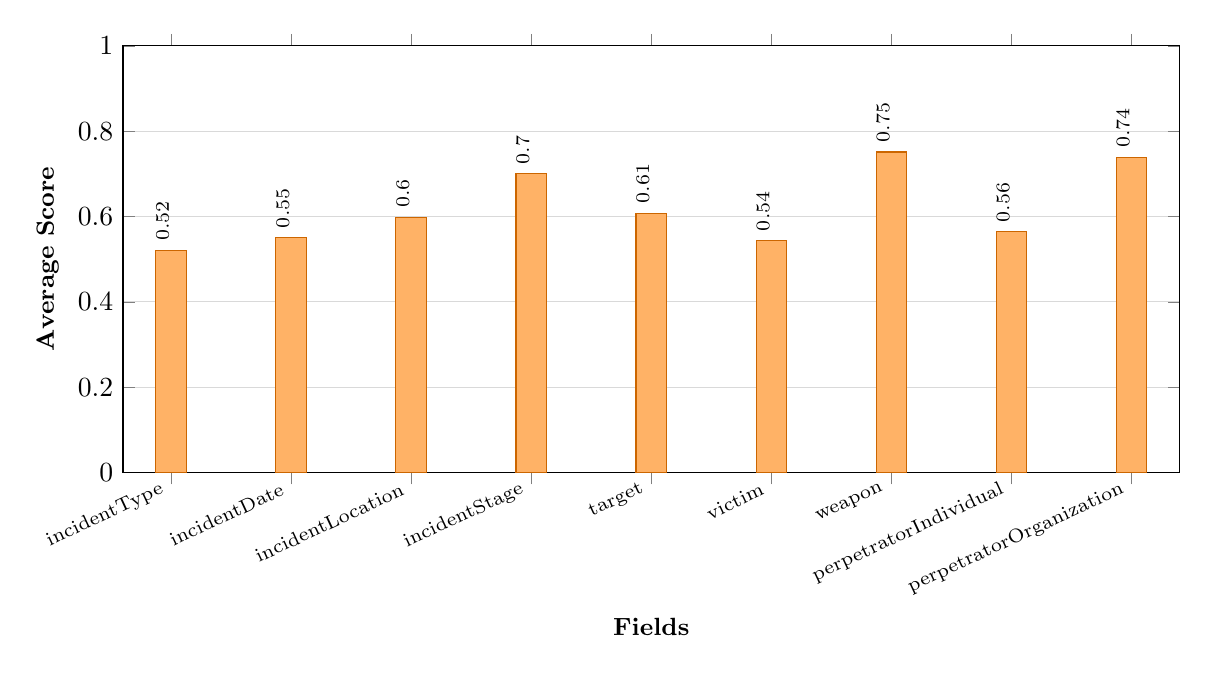
\begin{tikzpicture}
  \begin{axis}[
    width=15cm,
    height=7cm,
    ybar,
    bar width=11pt,
    ylabel={Average Score},
    ylabel style={font=\small\bfseries},
    xlabel={Fields},
    xlabel style={font=\small\bfseries},
    symbolic x coords={
      incidentType,
      incidentDate,
      incidentLocation,
      incidentStage,
      target,
      victim,
      weapon,
      perpetratorIndividual,
      perpetratorOrganization
    },
    xtick=data,
    xticklabel style={font=\scriptsize, rotate=25, anchor=east},
    ymin=0,
    ymax=1.0,
    ytick={0,0.2,0.4,0.6,0.8,1.0},
    ymajorgrids=true,
    grid style={line width=0.3pt, draw=gray!30},
    enlarge x limits=0.05,
    nodes near coords,
    nodes near coords style={font=\scriptsize, rotate=90, anchor=west, yshift=3pt}
  ]

  \addplot[fill=orange!60, draw=orange!80!black] coordinates {
    (incidentType, 0.520)
    (incidentDate, 0.550)
    (incidentLocation, 0.597)
    (incidentStage, 0.700)
    (target, 0.608)
    (victim, 0.543)
    (weapon, 0.751)
    (perpetratorIndividual, 0.564)
    (perpetratorOrganization, 0.738)
  };

  \end{axis}
\end{tikzpicture}

\caption{Per-field extraction performance for S2.1 on the MUC-4 subset ($N{=}100$). 
The iterative strategy shows uneven improvements across fields: structured categories such 
as \textit{weapon} and \textit{incidentStage} benefit most, whereas open-class fields like 
\textit{incidentType} and \textit{victim} remain comparatively challenging. These results 
illustrate how slot-wise prompting stabilizes certain fields while exposing residual 
difficulty in categories requiring interpretation or broader context.}
\label{fig:s2-perfield-plot}
\end{figure}


\subsection*{Latency}

Figure~\ref{fig:s2-latency-bar} shows that all S2 variants are comparatively fast, even though they issue one call per field. S2.0 is the speed leader, with a median latency of about $20$\,s per document and a tight upper tail (p99 below $50$\,s). Adding few-shot examples in S2.1 increases median latency to roughly $25$\,s and extends the tail (p99 around $72$\,s), but still keeps the strategy within a range that is substantially faster than the most accurate S1 configuration. S2.2, evaluated on speech-style inputs, sits between S2.0 and S2.1 in terms of latency: its median and mean latencies are slightly lower than S2.1, and its p99 value (about $53$\,s) is considerably shorter than S2.1’s, indicating more stable runtime behaviour. Overall, S2 provides an attractive accuracy–throughput trade-off: the strategy is noticeably faster than S1.1 and S3.1, while still achieving strong headline metrics.

\begin{figure}[H]
\centering
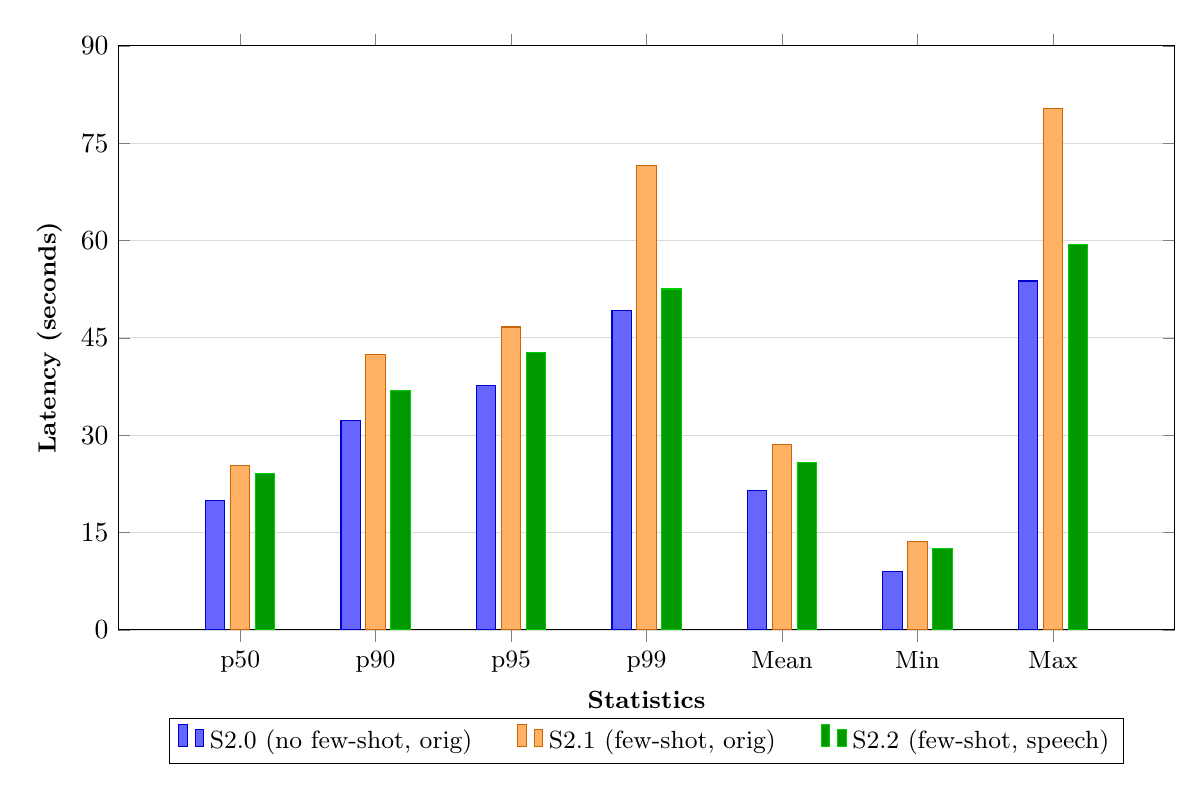
\begin{tikzpicture}
  \begin{axis}[
    width=15cm,
    height=9cm,
    ybar,
    bar width=7pt,
    ylabel={Latency (seconds)},
    ylabel style={font=\small\bfseries},
    xlabel={Statistics},
    xlabel style={font=\small\bfseries},
    symbolic x coords={p50, p90, p95, p99, Mean, Min, Max},
    xtick=data,
    xticklabel style={font=\small},
    ymin=0,
    ymax=90,
    ytick={0, 15, 30, 45, 60, 75, 90},
    ymajorgrids=true,
    grid style={line width=0.3pt, draw=gray!30},
    legend style={
      at={(0.5,-0.15)},
      anchor=north,
      legend columns=3,
      font=\small,
      /tikz/every even column/.append style={column sep=0.5cm}
    },
    enlarge x limits=0.15,
  ]
  
  % S2.0 (no few-shot, orig) - Blue
  \addplot[fill=blue!60, draw=blue!80!black] coordinates {
    (p50, 19.97)
    (p90, 32.24)
    (p95, 37.69)
    (p99, 49.26)
    (Mean, 21.48)
    (Min, 9.01)
    (Max, 53.76)
  };
  \addlegendentry{S2.0 (no few-shot, orig)}
  
  % S2.1 (few-shot, orig) - Orange
  \addplot[fill=orange!60, draw=orange!80!black] coordinates {
    (p50, 25.35)
    (p90, 42.48)
    (p95, 46.68)
    (p99, 71.52)
    (Mean, 28.58)
    (Min, 13.60)
    (Max, 80.28)
  };
  \addlegendentry{S2.1 (few-shot, orig)}
  
  % S2.2 (few-shot, speech) - Green
  \addplot[fill=green!60!black, draw=green!80!black] coordinates {
    (p50, 24.07)
    (p90, 36.93)
    (p95, 42.81)
    (p99, 52.53)
    (Mean, 25.83)
    (Min, 12.51)
    (Max, 59.36)
  };
  \addlegendentry{S2.2 (few-shot, speech)}
  
  \end{axis}
\end{tikzpicture}
\caption{Latency statistics for S2 variants (seconds). The plot compares execution times for S2.0 (no few-shot), S2.1 (few-shot), and S2.2 (few-shot with speech-style input). S2.1 shows the highest latency because few-shot prompts increase token processing, while S2.0 remains the fastest. The speech-style variant (S2.2) reduces extreme latencies relative to S2.1, suggesting that prompt length impacts cost more than input complexity. Overall, the results illustrate the trade-off between improved accuracy from few-shot prompting and the computational overhead of iterative, slot-wise extraction.}
\label{fig:s2-latency-bar}
\end{figure}


\subsection*{Cost Analysis (S2: Single-Field Iterative)}

\textbf{Assumptions.} Each of the $F{=}9$ MUC-4 slots is extracted with a separate \textit{GPT-5} call. Per field, the average token usage is $i_f{=}1{,}500$ input tokens and $o_f{=}50$ output tokens. Verification with \textit{GPT-5-mini} is performed once per record (not per field) with $V_{\text{in}}{=}1{,}000$ and $V_{\text{out}}{=}100$. If audio is used, Whisper transcription for $D$ minutes is added once per record.

\textbf{Prices.} GPT-5: input \$1.25/M, output \$10.00/M. GPT-5-mini: input \$0.25/M, output \$2.00/M. Whisper: \$0.006/min.

\textbf{Formula.}
\[
\text{Cost}_{\text{S2}} =
\underbrace{
\sum_{f=1}^{F}\!\left(\frac{i_f}{10^6}p_{\text{in}}+\frac{o_f}{10^6}p_{\text{out}}\right)
}_{\text{per-field extraction on GPT-5}}
+
\underbrace{
\frac{V_{\text{in}}}{10^6}p^{(\text{mini})}_{\text{in}}+\frac{V_{\text{out}}}{10^6}p^{(\text{mini})}_{\text{out}}
}_{\text{single verification on GPT-5-mini}}
+0.006\cdot D
\]

\textbf{Per-record (no audio).}
\[
9\times\Big(
\underbrace{\tfrac{1500}{10^6}\!\cdot\!1.25}_{\$0.001875}
+\underbrace{\tfrac{50}{10^6}\!\cdot\!10.00}_{\$0.000500}
\Big)
+\underbrace{\tfrac{1000}{10^6}\!\cdot\!0.25}_{\$0.000250}
+\underbrace{\tfrac{100}{10^6}\!\cdot\!2.00}_{\$0.000200}
=\mathbf{\$0.02183}\ (\approx 2.18\text{¢/doc})
\]

\textbf{With audio (Whisper).} Adding Whisper introduces a linear term of $0.006\cdot D$. For $D{=}1$\,min, the total cost becomes $\$0.02183 + 0.006 = \mathbf{\$0.02783}$ (approximately $2.78$\,¢ per document). Under the assumed token budgets, S2 therefore costs about $3.0\times$ as much as S1 (\$0.02183 vs.\ \$0.00720 per document, no audio), driven by the $F$ separate extraction calls; running verification only once per record keeps the arbiter overhead comparatively small.

\subsection*{Consistency (Formatting \& Style)}

Figure~\ref{fig:s2-consistency} indicates that the iterative strategy maintains very high schema conformity and stable style. All variants achieve $\mathrm{FPR}_{\text{overall}} \geq 0.940$, with S2.0 reaching $0.970$, which reflects that the per-field design and explicit JSON schemas make it easy for the model to respect structural constraints. The style-aware score $\mathrm{SC}_{\text{macro}}$ modestly improves from $0.672$ in S2.0 to $0.683$ in S2.1, suggesting that few-shot prompts help the model settle on more consistent textual realizations across documents. S2.2, evaluated on speech-style input, shows a small drop in both metrics but remains close to S2.1, which indicates that formatting and style are largely preserved even when the input becomes noisier. Taken together with the headline metrics, this suggests that S2 trades a slight reduction in schema strictness (relative to S2.0) for better content accuracy and calibration in S2.1, and that these gains mostly carry over to spoken-like transcripts in S2.2.

Overall, the S2 family occupies a middle ground between single-pass and full consensus strategies. Iterative, field-specific prompting improves challenging slots such as \texttt{incidentLocation}, while still struggling with intrinsically difficult fields like \texttt{perpetratorIndividual}. Few-shot prompting (S2.1) clearly improves accuracy and reduces hallucinations compared to S2.0, at the cost of a moderate latency and cost increase. The speech-style variant S2.2 preserves much of this behaviour on noisier inputs, with strong RFA and only modest degradation in calibration metrics. Compared to S1.1, S2.1 offers similar or slightly lower headline scores on clean text but achieves substantially better throughput; compared to S3.1 and S4.1, it provides a simpler and more economical alternative that still benefits from per-field control, making it a compelling choice for deployments where latency and cost are constrained but field-level interpretability is desirable.

\begin{figure}[H]
\centering
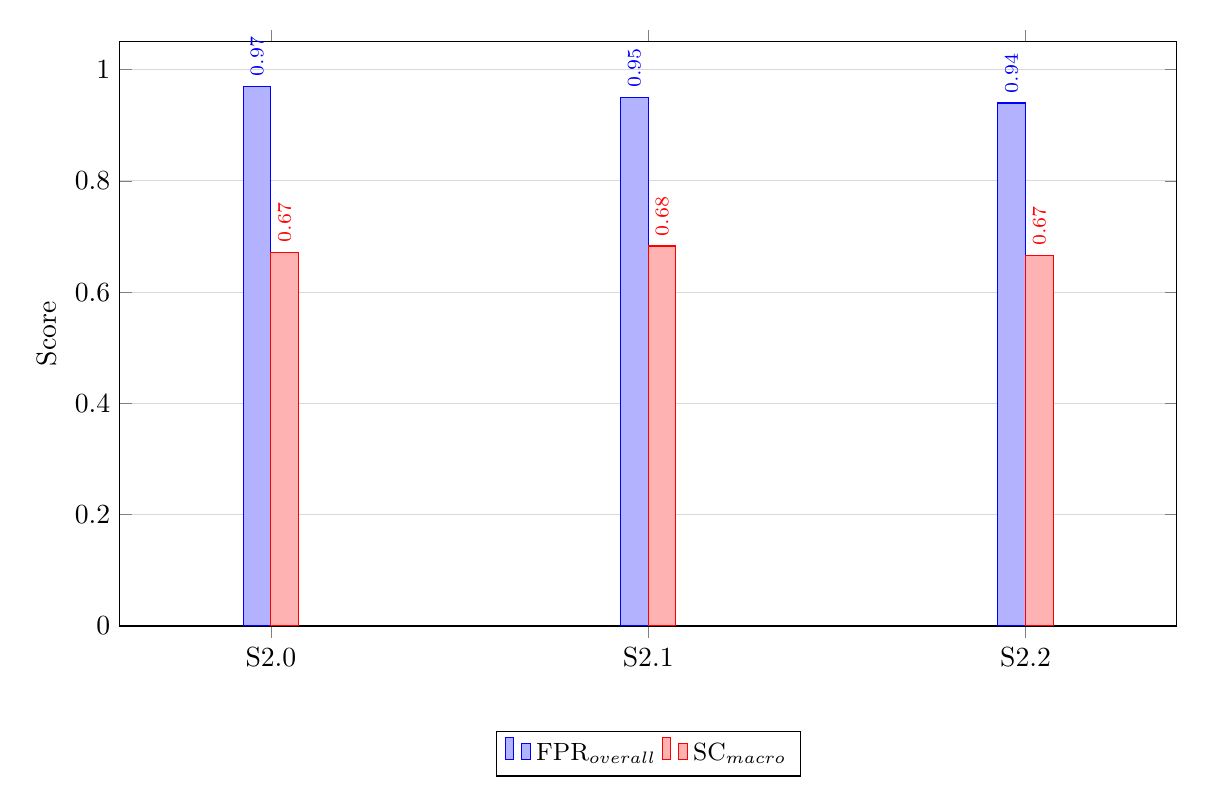
\begin{tikzpicture}
  \begin{axis}[
    width=15cm,
    height=9cm,
    ybar=0pt,
    bar width=10pt,
    ymin=0, ymax=1.05,
    ylabel={Score},
    symbolic x coords={S2.0,S2.1,S2.2},
    xtick=data,
    ymajorgrids=true,
    grid style={line width=0.3pt, draw=gray!30},
    legend style={at={(0.5,-0.18)}, anchor=north, legend columns=2, font=\small},
    enlarge x limits=0.20,
    nodes near coords,
    nodes near coords style={
        font=\scriptsize,
        rotate=90,
        anchor=west,
    }
  ]

    % FPR_overall
    \addplot coordinates {(S2.0,0.970) (S2.1,0.950) (S2.2,0.940)};
    \addlegendentry{$\mathrm{FPR}_{\text{overall}}$}

    % SC_macro
    \addplot coordinates {(S2.0,0.672) (S2.1,0.683) (S2.2,0.666)};
    \addlegendentry{$\mathrm{SC}_{\text{macro}}$}

  \end{axis}
\end{tikzpicture}
\caption{Consistency (S2 variants): schema formatting vs.\ input-aware style.}
\label{fig:s2-consistency}
\end{figure}

